\documentclass[11pt,a4paper]{article}

\usepackage[utf8]{inputenc}
\usepackage[T1]{fontenc}
\usepackage{newtxtext,newtxmath}
\usepackage[margin=1in]{geometry}
\usepackage{microtype}
\usepackage{graphicx}
\usepackage{booktabs}
\usepackage{tabularx}
\usepackage{longtable}
\usepackage{array}
\usepackage{enumitem}
\usepackage[font=small,labelfont=bf,labelsep=period]{caption}
\usepackage{float}
\usepackage{titlesec}
\usepackage[hidelinks]{hyperref}

\setlist{itemsep=2pt,topsep=4pt,parsep=0pt}
\setlength{\parindent}{0pt}
\setlength{\parskip}{5pt}
\renewcommand{\arraystretch}{1.2}
\captionsetup[table]{position=above,skip=5pt,justification=raggedright,singlelinecheck=false}
\captionsetup[figure]{position=below,skip=5pt}

\titleformat{\section}{\large\bfseries}{}{0pt}{}
\titleformat{\subsection}{\normalsize\bfseries}{}{0pt}{}
\titleformat{\subsubsection}{\normalsize\itshape\bfseries}{}{0pt}{}
\titlespacing*{\section}{0pt}{14pt}{6pt}
\titlespacing*{\subsection}{0pt}{10pt}{4pt}
\titlespacing*{\subsubsection}{0pt}{8pt}{3pt}

\newcolumntype{R}{>{\raggedleft\arraybackslash}X}
\newcolumntype{L}{>{\raggedright\arraybackslash}X}
\newcommand{\hd}[1]{\textbf{#1}}
\newcommand{\tablestyle}{\small}
\newcommand{\headrow}{}
\newenvironment{hangparagraph}{\par\setlength{\leftskip}{1.2cm}\setlength{\parindent}{-1.2cm}}{\par}

\begin{document}

\begin{center}
{\LARGE\bfseries When Should Past Behaviour Shape Search?\par}
\vspace{6pt}
{\large Personalised Re-ranking on the JDsearch Dataset\par}
\vspace{10pt}
{BT4222 Project Interim Report\par}
\vspace{10pt}
{\bfseries Group 17\par}
\vspace{4pt}
ARIFOVAS KRISTUPAS \quad KUNERT LIAM\\
YANG BRIAN CHEN \quad YILDIRIM MICHEL\par
\vspace{6pt}
4 October 2026
\end{center}
\vspace{4pt}

%==============================================================
\section{Part 1. Machine Learning Problem}

\begin{itemize}
\item \textbf{Business objective.} For each search, the dataset records about 90 candidate products displayed by JD's search engine, but shoppers who type the same query differ in the brands, shops and product types they prefer. Ranking each shopper's likely choices higher helps them find and buy suitable products sooner. Over-personalising is also a risk, because past favourites can crowd out what the query asks for. The business decision is therefore how much a shopper's past behaviour should influence the current ranking, and which parts of that history to trust.

\item \textbf{ML alignment.} This maps to personalised re-ranking: score every candidate JD returned for a search and sort by score. Offline ranking quality is the measurable proxy; revenue and satisfaction are not observed in the data.

\item \textbf{Question the model must answer.} Which historical signals (same product, shop, brand, category depth, action type, recency; search-linked versus query-less history) improve the ranking of the current search, and does weighting history by its relevance to the query outperform using all of it equally or filtering it?

\item \textbf{Input sample.} One (search, candidate) pair, scored within its complete candidate list. Inputs are the current query (anonymised term IDs); the shopper's history (products, action types CLICK/CART/FLW/ORD, the query behind each action, and time gaps); and candidate metadata (title terms, brand, four-level category, shop). All candidates of one search form one ranking group and stay together when sampling or splitting.

\item \textbf{Target.} The graded label of each candidate: 0 = no interaction, 1 = click, 2 = add to cart, 3 = purchase, used as the relevance gain.

\item \textbf{Evaluation.} NDCG@10 on complete, un-downsampled candidate lists, with MRR and Recall@10 as supporting metrics. The 2,103 searches (1.2\%) without any engaged candidate are excluded from evaluation, following the source paper, because every ordering scores identically on them. Accuracy is unsuitable: 97.9\% of candidate labels are 0.
\end{itemize}

%==============================================================
\section{Part 2. Dataset and Impression Data Understanding}

\subsection{2.1 Data Overview and Sampling Scheme}

\textbf{Source.} JDsearch (Liu et al., 2023) contains real, anonymised product-search logs from JD.com. The behaviour file holds one record per sampled active user: their last search, the candidates shown with outcome labels, and their earlier interaction history. A separate catalogue describes products. All text (queries, titles, brand and category names) is replaced by term IDs: term boundaries are recoverable, meanings are not.

\begin{table}[H]
\caption{Dataset scale (full data)}
\tablestyle
\centering
\begin{tabularx}{0.85\textwidth}{L R}
\toprule
\headrow \hd{Entity} & \hd{Count} \\
\midrule
Search records (one per sampled user) & 173,831 \\
Distinct current queries & 111,556 \\
Candidate occurrences (impressions) & 15,510,012 \\
Distinct candidate products & 8,362,535 \\
Historical actions & 26,667,260 \\
Distinct products in histories & 5,584,543 \\
Products in catalogue & 12,141,247 \\
Behaviour products missing from catalogue & 731,389 \\
Brands / shops & 182,585 / 250,934 \\
Category IDs at levels 1 / 2 / 3 / 4 & 76 / 671 / 5,819 / 7,137 \\
Current-query vocabulary (distinct term IDs) & 47,461 \\
Collection period & 18 Oct 2021 -- 17 Oct 2022 \\
\bottomrule
\end{tabularx}
\end{table}

Catalogue metadata is available for 99.6\% of candidate occurrences and 95.1\% of historical actions. Including the 731,389 behaviour products missing from the catalogue, the product universe totals 12,872,636, matching the paper.

\textbf{Time span.} Histories cover 18 October 2021 to 17 October 2022, and all final searches occur on 17 October 2022 (Liu et al., 2023, \S3.1). The file stores relative gaps rather than timestamps. Read as seconds, the gaps give a median history span of 283 days, a 95th percentile of 362 days and only one record above 365 days. This is consistent with the documented one-year window, so we treat gaps as seconds.

\textbf{Sampling scheme.}
\begin{itemize}
\item Raw statistics (Sections 2.1--2.2) use the full files, streamed record by record; no counts are estimated.
\item Engineered-feature statistics (Sections 2.3--2.4) use a uniform random sample of 5,000 complete search records (seed 4222). It holds 449,052 candidates with all history retained, and metadata is looked up in the full catalogue. Table 2 shows that the sample matches the full data.
\item Modelling will split by whole search record. All final searches share one date and rows carry no absolute timestamps, so a cross-user temporal split is not meaningful. The 5,000 records explored here have already informed our feature choices, which we will keep in mind when setting up the final evaluation.
\end{itemize}

\begin{table}[H]
\caption{Exploration sample versus full data}
\tablestyle
\centering
\begin{tabularx}{0.9\textwidth}{L R R}
\toprule
\headrow \hd{Measure} & \hd{Full data} & \hd{5,000-record sample} \\
\midrule
Search records & 173,831 & 5,000 \\
Candidate occurrences & 15,510,012 & 449,052 \\
Mean candidates per search & 89.2 & 89.8 \\
Median history length (actions) & 78 & 75 \\
Share of candidates engaged (label $\geq$ 1) & 2.07\% & 2.08\% \\
Share of candidates purchased (label 3) & 0.134\% & 0.134\% \\
\bottomrule
\end{tabularx}
\end{table}

%--------------------------------------------------------------
\subsection{2.2 Impression, Exposure and Interaction Dynamics}

Every candidate is an impression: a product shown to the user for the current query. The properties below determine how we construct features, labels and evaluation.

\subsubsection{(a) Impression slates}

Searches show a median of 90 candidates (mean 89.2, standard deviation 38.9); 90\% show between 25 and 170, within a range of 1 to 200 (Figure 1). A top-10 ranking therefore selects roughly one in nine shown products.

\begin{figure}[H]
\centering
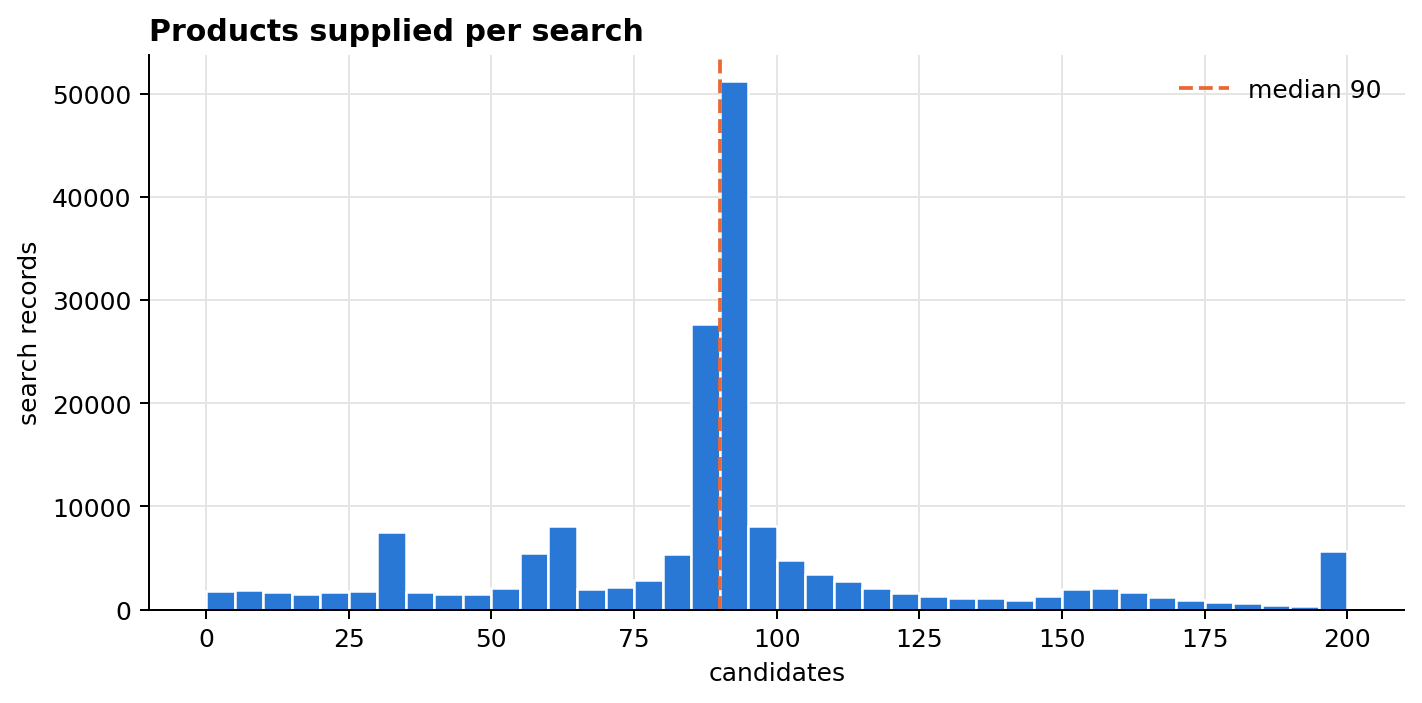
\includegraphics[width=0.75\textwidth]{figures/fig1_slate_length.png}
\caption{Candidates supplied per search (full data)}
\end{figure}

\subsubsection{(b) Position and candidate order}

In 100\% of searches containing an engaged candidate, every engaged candidate precedes every non-engaged one in the file. Engagement is 99\% at file position 1 and near zero beyond position 10 (Figure 2). File order therefore encodes the label rather than the displayed rank, so click-through rate by display position cannot be computed. Candidate position is excluded from all features, and evaluation breaks score ties at random; using file order would leak the label.

\begin{figure}[H]
\centering
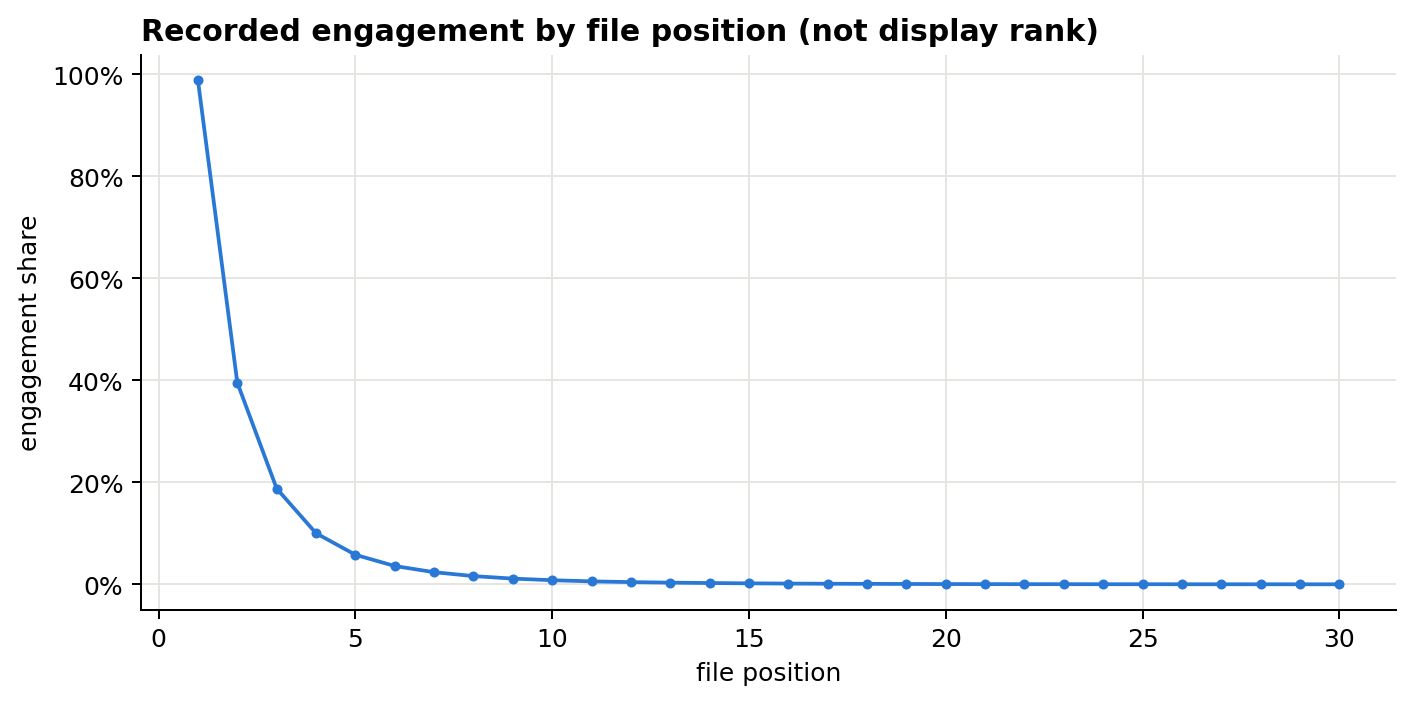
\includegraphics[width=0.75\textwidth]{figures/fig2_position_artifact.png}
\caption{Engagement share by file position: a storage artefact, not display rank}
\end{figure}

\subsubsection{(c) Interaction hierarchy}

Each candidate records its deepest outcome. Exclusively, 224,487 candidates are clicks (1.45\%), 75,573 carts (0.49\%), 20,836 purchases (0.13\%) and 15,189,116 have no interaction (97.93\%). Table 3 shows the cumulative levels.

\begin{table}[H]
\caption{Interaction depth (full data)}
\tablestyle
\centering
\begin{tabularx}{\textwidth}{L R R R}
\toprule
\headrow \hd{Outcome level} & \hd{Candidates} & \hd{Share of candidates} & \hd{Searches containing it} \\
\midrule
Shown & 15,510,012 & 100\% & 100\% \\
Any engagement (label $\geq$ 1) & 320,896 & 2.07\% & 98.8\% \\
Cart or purchase (label $\geq$ 2) & 96,409 & 0.62\% & 42.2\% \\
Purchase (label 3) & 20,836 & 0.13\% & 11.7\% \\
\bottomrule
\end{tabularx}
\end{table}

Of engaged candidates, 30.0\% reach cart or purchase and 6.5\% reach purchase. Because labels record only the deepest outcome, these are depth-of-engagement shares, not observed click-to-cart-to-purchase conversion rates. Nearly every search (98.8\%) contains an engaged candidate because the dataset samples users' last searches; this is a property of the sample, not JD's overall search conversion.

\subsubsection{(d) Feedback semantics}

\begin{table}[H]
\caption{Types of feedback and their use}
\tablestyle
\centering
\begin{tabularx}{\textwidth}{>{\raggedright\arraybackslash}p{3.3cm} R L L}
\toprule
\headrow \hd{Signal} & \hd{Count} & \hd{Interpretation} & \hd{Use in modelling} \\
\midrule
Shown, engaged (label 1--3) & 320,896 & Positive, graded by depth & Graded positive \\
Shown, not engaged (label 0) & 15,189,116 & Shown without interaction; may not have been examined; not an explicit dislike & Negative within its own list \\
Not shown in this search & Not countable & Unobserved: no exposure, no preference & Never used as a negative \\
Past action in history & 26,667,260 & Recorded positive action; no past ignored items & Preference evidence \\
\bottomrule
\end{tabularx}
\end{table}

Label-0 candidates are genuine exposed-but-unengaged negatives, so ranking can be learned within each list without inventing negatives from unseen products. Products not shown in a search are unobserved: 3,835,625 catalogue products appear in no candidate list at all. History contains only positive actions, with no record of what was shown but ignored in the past.

\subsubsection{(e) Sparsity}

\begin{itemize}
\item \textbf{History length:} median 78 actions, mean 153, 95th percentile 548 and maximum 4,802, a long tail of heavy users.
\item \textbf{Action mix:} cart 43.2\%, click 31.1\%, purchase 25.6\%, follow 0.1\%. Carts outnumber clicks in history although clicks dominate candidate labels, so action types carry different evidence and should not share fixed weights.
\item \textbf{Query-less history:} 64.7\% of past actions have no recorded query (for example, browsing or recommendations), so most preference evidence comes from outside search.
\item \textbf{Item popularity:} 75.2\% of distinct candidates appear in only one search's list. The top 1\% of candidates receive 14.3\% of exposures, while the top 1\% of history products account for 34.9\% of actions (Figure 3).
\item \textbf{Cold items:} 56.5\% of candidate occurrences (80.5\% of distinct candidates) never appear in any history. Product-ID embeddings get few or no training examples for these items, which motivates brand, shop, category and title features.
\end{itemize}

\begin{figure}[H]
\centering
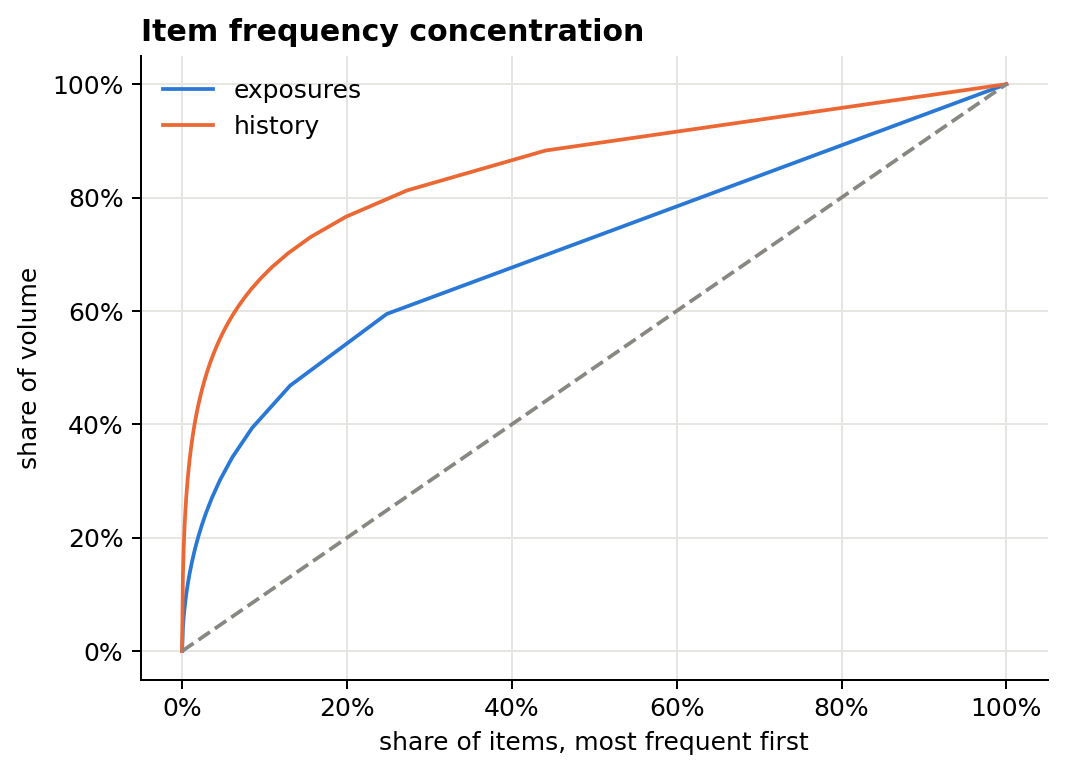
\includegraphics[width=0.55\textwidth]{figures/fig3_item_popularity.png}
\caption{Concentration of item frequency in exposures and histories (full data)}
\end{figure}

\subsubsection{(f) Temporal patterns}

Gaps between consecutive past actions have a median of 67 seconds, an upper quartile of about 2.1 hours and a 95th percentile of about 6.8 days; 10.6\% are zero (actions logged together). The gap from the last action to the current search has a median of about 5.4 hours and a 95th percentile of about 26 days (Figure 4). Behaviour is bursty, with short sessions separated by long breaks, which motivates testing recency-weighted features.

\begin{figure}[H]
\centering
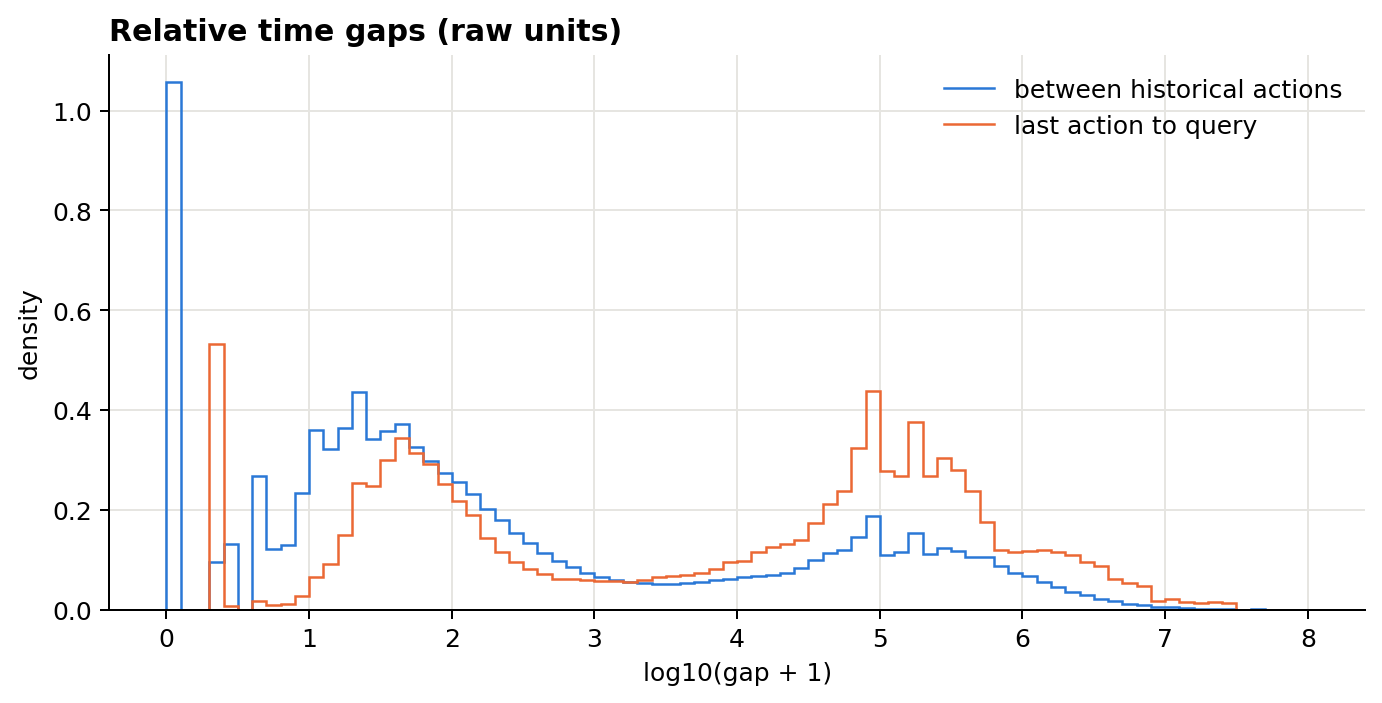
\includegraphics[width=0.75\textwidth]{figures/fig4_time_gaps.png}
\caption{Distribution of time gaps, log scale (full data)}
\end{figure}

%--------------------------------------------------------------
\subsection{2.3 Feature Dictionary and Descriptive Statistics}

Table 5 lists the released fields. From them we engineered 48 features in six families (Table 6), computed on the 5,000-record sample; the complete dictionary is in Appendix A. Search-level features are constant within a candidate list, so they can change a ranking only by modulating candidate-level signals.

\begin{table}[H]
\caption{Raw fields}
\tablestyle
\centering
\begin{tabularx}{\textwidth}{>{\ttfamily\small\raggedright\arraybackslash}p{3.4cm} l L L}
\toprule
\headrow \hd{Field} & \hd{File} & \hd{Description} & \hd{Type / unit} \\
\midrule
query & Behaviour & Current search query & Text (term IDs) \\
candidate\_wid\_list & Behaviour & Products shown for the query & List of product IDs \\
candidate\_label\_list & Behaviour & Outcome per candidate: 0 none, 1 click, 2 cart, 3 purchase & List of ordinal labels \\
history\_qry\_list & Behaviour & Query behind each past action; -1 = not from search & List of text / -1 \\
history\_wid\_list & Behaviour & Product of each past action & List of product IDs \\
history\_type\_list & Behaviour & CLICK, CART, FLW (follow), ORD (purchase) & List of categories \\
history\_time\_list & Behaviour & Gap to previous action; final value = gap to current search & List of integers (seconds) \\
wid & Catalogue & Product ID & Categorical ID \\
name & Catalogue & Product title & Text (term IDs) \\
brand\_id, brand\_name & Catalogue & Brand & Categorical ID, text \\
cate\_id\_1..4, cate\_name\_1..4 & Catalogue & Four-level category & Categorical ID, text \\
shop\_id & Catalogue & Seller shop & Categorical ID \\
\bottomrule
\end{tabularx}
\end{table}

\begin{table}[H]
\caption{Engineered feature families (5,000-record sample)}
\tablestyle
\centering
\begin{tabularx}{\textwidth}{>{\raggedright\arraybackslash}p{2.5cm} l r L L}
\toprule
\headrow \hd{Family} & \hd{Level} & \hd{No.} & \hd{Examples} & \hd{Captures} \\
\midrule
Search context & Search & 14 & History length and span; action counts by type; share of history without a query; metadata coverage; query length; time since last action; list length & Who searches, and how \\
History--query overlap & Search & 3 & Max Jaccard; any overlap; identical term set & Whether a similar search occurred before \\
Query--product match & Candidate & 5 & Shared title terms; coverage; Jaccard; brand-name and category-name match & Lexical relevance \\
Exact repeat & Candidate & 5 & Seen before; ordered before; past actions on the product (all, search-linked, query-less) & Prior interest in this product \\
Attribute affinity & Candidate & 18 & Past actions on the same brand, shop and category path L1--L4, each from all, search-linked and query-less history & Broader preferences \\
Popularity and coverage & Candidate & 3 & History popularity; cold flag; in-catalogue flag & Head versus long tail \\
Planned & Candidate & -- & Recency-weighted and action-weighted affinity & To be tested in modelling \\
\bottomrule
\end{tabularx}
\end{table}

Table 7 reports statistics for representative features. Values are missing where candidate metadata is unavailable (1,960 candidates) and, for shop features, also where the shop ID is absent (5,963 in total); they are kept as missing rather than treated as non-matches.

\begin{table}[H]
\caption{Numeric statistics, representative features (5,000 searches; 449,052 candidates)}
\tablestyle
\centering
\setlength{\tabcolsep}{4pt}
\begin{tabularx}{\textwidth}{>{\raggedright\arraybackslash}p{4.6cm} l r r r r r r}
\toprule
\headrow \hd{Feature} & \hd{Level} & \hd{Min} & \hd{Max} & \hd{Mean} & \hd{Median} & \hd{Std} & \hd{Missing} \\
\midrule
History length (actions) & Search & 1 & 3,662 & 151.7 & 75 & 231.0 & 0 \\
Share of history without query & Search & 0 & 1 & 0.60 & 0.61 & 0.20 & 0 \\
Time since last action (hours) & Search & 0.0003 & 8,696.6 & 140.7 & 5.7 & 563.3 & 0 \\
Query length (terms) & Search & 1 & 46 & 2.77 & 2 & 1.90 & 0 \\
Max history--query Jaccard & Search & 0 & 1 & 0.17 & 0 & 0.23 & 0 \\
Query--title coverage & Cand. & 0 & 1 & 0.72 & 1.00 & 0.34 & 1,960 \\
Query--title Jaccard & Cand. & 0 & 1 & 0.077 & 0.067 & 0.058 & 1,960 \\
Past actions, same product & Cand. & 0 & 107 & 0.019 & 0 & 0.41 & 0 \\
Past actions, same brand & Cand. & 0 & 444 & 2.47 & 0 & 13.1 & 1,960 \\
Past actions, same shop & Cand. & 0 & 316 & 0.49 & 0 & 4.71 & 5,963 \\
Past actions, same L1 path & Cand. & 0 & 2,216 & 26.8 & 5 & 78.1 & 1,960 \\
Past actions, same L4 path & Cand. & 0 & 546 & 5.57 & 0 & 23.3 & 1,960 \\
Popularity in all histories & Cand. & 0 & 44,063 & 33.5 & 0 & 346.0 & 0 \\
\bottomrule
\end{tabularx}
\end{table}

Categorical fields are high-cardinality anonymised IDs, so Table 8 reports concentration rather than example values. 17 level-3 and 33 level-4 category IDs occur under more than one parent, so category features match the full ancestor path.

\begin{table}[H]
\caption{Categorical fields (full data)}
\tablestyle
\centering
\begin{tabularx}{0.9\textwidth}{L R R R}
\toprule
\headrow \hd{Field} & \hd{Distinct values} & \hd{Most common value's share} & \hd{Missing} \\
\midrule
Brand ID & 182,585 & 4.3\% & 0 \\
Shop ID & 250,934 & 0.13\% & 103,162 \\
Category L1 / L2 & 76 / 671 & 9.2\% / 3.7\% & 0 \\
Category L3 / L4 & 5,819 / 7,137 & 1.3\% / 1.3\% & 0 \\
History action type & 4 & 43.2\% (CART) & 0 \\
Candidate label & 4 & 97.9\% (label 0) & 0 \\
\bottomrule
\end{tabularx}
\end{table}

\begin{table}[H]
\caption{Text lengths in term IDs (full data)}
\tablestyle
\centering
\begin{tabularx}{0.9\textwidth}{L R R R R R}
\toprule
\headrow \hd{Text} & \hd{Count} & \hd{Median} & \hd{Mean} & \hd{95th pct.} & \hd{Max} \\
\midrule
Current query & 173,831 & 2 & 2.75 & 5 & 58 \\
Past query (excluding -1) & 9,402,709 & 2 & 2.68 & 5 & 1,441 \\
Product title & 12,141,247 & 27 & 27.9 & 42 & 78 \\
Brand name (non-empty) & 11,199,587 & 2 & 2.56 & 5 & 31 \\
Category L3 name & 12,141,247 & 2 & 1.91 & 4 & 15 \\
\bottomrule
\end{tabularx}
\end{table}

The current-query vocabulary contains 47,461 distinct term IDs. Queries are short (median 2 terms) and titles long (median 27), so query--title overlap compares a few terms against a long description. Population features (history popularity, cold flag) use the full data here for description only; in modelling they will be derived from training records only, to avoid leaking test information.

%--------------------------------------------------------------
\subsection{2.4 Early Signal Checks and Modelling Implications}

To test which signals carry ranking information before modelling, we ranked each sampled search by a single feature and measured NDCG@10 against random ordering. The test uses 4,941 sampled searches with at least one engaged candidate, linear gains 0--3, complete lists and random tie-breaking. Paired bootstrap 95\% intervals (2,000 resamples) are reported for key differences. These are untrained heuristics: they show which signals exist, not the gain of a trained model.

\begin{figure}[H]
\centering
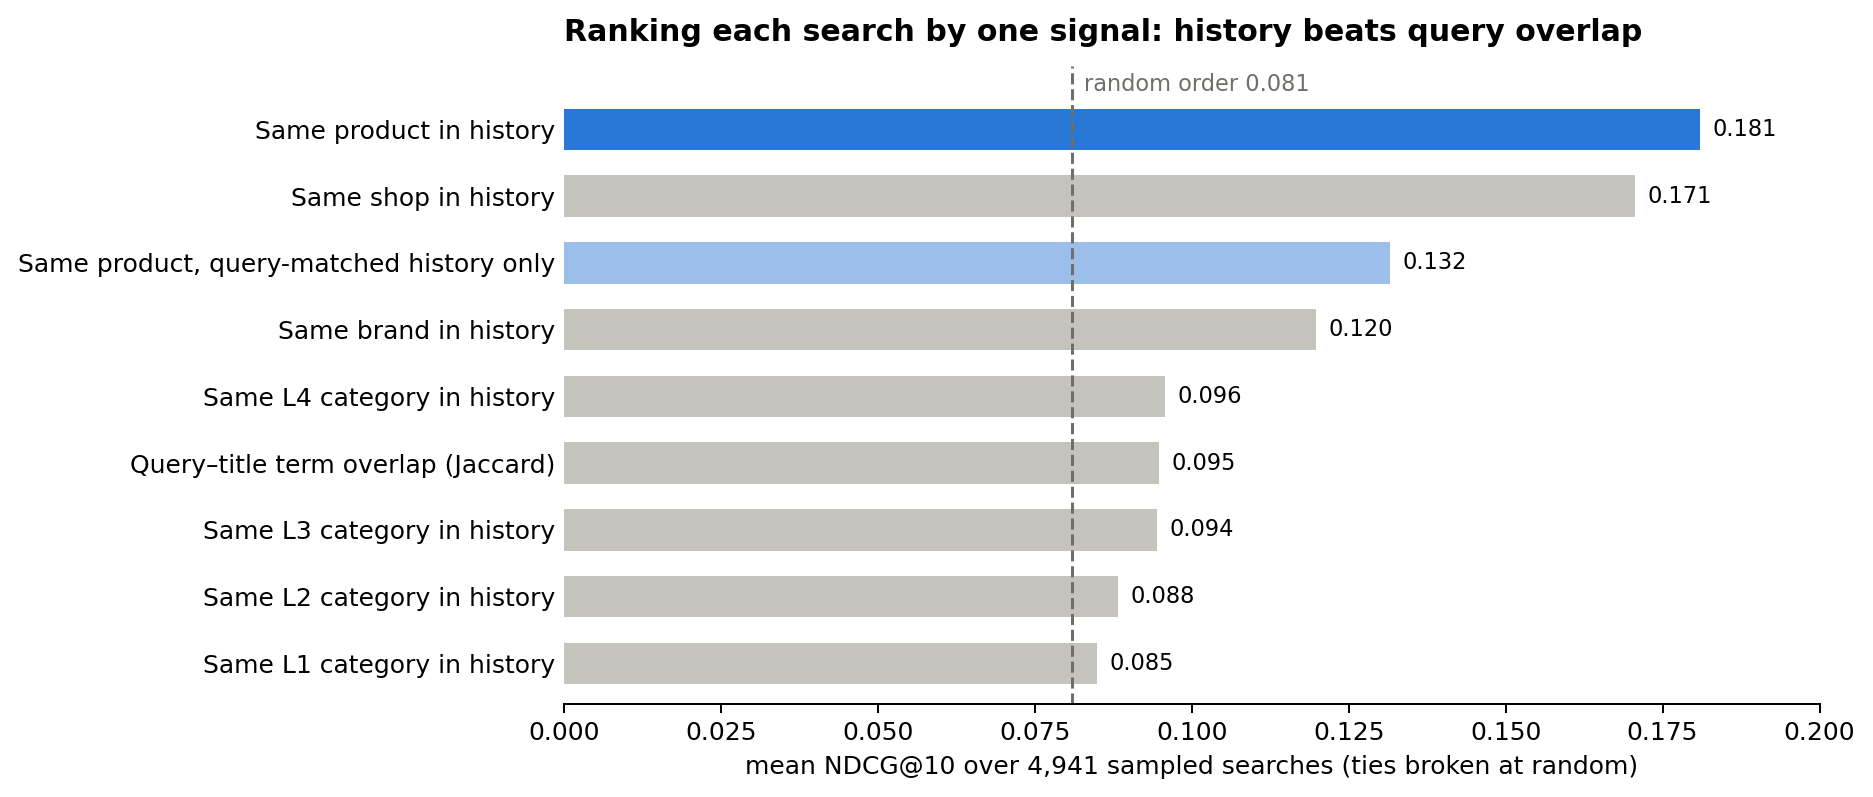
\includegraphics[width=\textwidth]{figures/fig5_signal_ndcg.png}
\caption{NDCG@10 of one-signal rankings versus random order (5,000-record sample)}
\end{figure}

\begin{enumerate}
\item \textbf{Exact repeats are strong but rare.} Same-product history scores 0.181 (random 0.081) but covers only 0.79\% of candidates; matched candidates are engaged 25.8\% of the time versus 1.9\% otherwise. It is a key feature but cannot carry a model alone.
\item \textbf{Shop and brand history are broader signals.} Shop scores 0.171 at 7.2\% coverage and brand 0.120 at 22.7\% coverage. Attribute-level evidence can also reach products the shopper has never interacted with (part of the signal still comes from exact repeats), which matters because 56.5\% of candidates are cold.
\item \textbf{Hard-filtering history by the query hurts.} Restricting same-product evidence to past actions whose query overlaps the current one lowers NDCG@10 from 0.181 to 0.132 (95\% interval of the drop: 0.044 to 0.055). A hard filter discards useful evidence, including all query-less history, which has no query to overlap; this motivates comparing query-aware soft weighting with using all history.
\item \textbf{Query-less history carries signal.} Same-product evidence from query-less history alone scores 0.150, versus 0.140 from search-linked history, so both sources are retained.
\item \textbf{Query--title overlap is a real but modest signal.} Jaccard overlap scores 0.095 (gain over random: 0.009 to 0.019). JD's retrieval already returns lexically relevant products, so personal history has more room to add ranking value.
\item \textbf{Category depth adds little beyond L3.} Scores rise from 0.085 at L1 to 0.096 at L4, but L4 adds only 0.0013 over L3 (interval 0.0004 to 0.0022). Full category paths will be used, but depth is not a central claim.
\end{enumerate}

%==============================================================
\section{Part 3. Limitations and Next Steps}

\subsection{3.1 Limitations}

\begin{enumerate}
\item \textbf{No display rank.} File order encodes outcomes, so position bias cannot be studied or corrected.
\item \textbf{No persistent user IDs or absolute timestamps.} Each record is one user's last search, so no cross-user temporal split is possible.
\item \textbf{Anonymised text.} Terms can be matched but not interpreted; related queries without shared terms appear unrelated.
\item \textbf{Selected sample.} Records are active users' last searches, almost all containing an engagement; rates do not represent JD's overall traffic.
\item \textbf{Missing metadata.} 4.9\% of historical actions and 0.4\% of candidates lack catalogue information, which can hide genuine matches.
\item \textbf{Outcome-only labels.} Labels record the deepest action, not the interaction path, revenue or explicit dislikes.
\end{enumerate}

\subsection{3.2 Next Steps}

\begin{enumerate}
\item \textbf{Reproduce and diagnose the prior baseline.} Team 3 built an LSTM-with-attention and NCF hybrid. We will re-evaluate it under our protocol (complete lists, NDCG@10, label-independent candidate order) and diagnose:
  \begin{itemize}
  \item negatives downsampled to four per positive, which inflates ranking scores;
  \item 4-class classification judged by accuracy and F1, under which the unweighted model predicted class 0 for 98.7\% of samples;
  \item no use of the current query, so history attention is not conditioned on it;
  \item possible leakage of the positive-first candidate order into training or evaluation.
  \end{itemize}
\item \textbf{Simple baselines:} random order, popularity, and the one-signal rules in Section 2.4.
\item \textbf{Feature-based ranker:} a learning-to-rank model over the Section 2.3 feature families, chosen after the baseline comparisons.
\item \textbf{Controlled comparisons:} no history versus all history versus hard filtering versus query-aware soft weighting, plus recency and action-type weights, reported separately for cold and warm candidates and for short and long histories. The no-history model (query--product match, candidate metadata, training-set popularity) is the reference that isolates what personalisation adds.
\end{enumerate}

Query-aware history models already exist; the JDsearch paper itself benchmarks several (Liu et al., 2023). Our contribution is therefore a corrected evaluation of the prior baseline and controlled evidence on when, and how strongly, history should influence search ranking.

%==============================================================
\section*{References}

\begin{hangparagraph}
Liu, J., Dou, Z., Tang, G., \& Xu, S. (2023). JDsearch: A personalized product search dataset with real queries and full interactions. In \textit{Proceedings of the 46th International ACM SIGIR Conference on Research and Development in Information Retrieval (SIGIR '23)}. \url{https://arxiv.org/abs/2305.14810}
\end{hangparagraph}

\begin{hangparagraph}
Liu, J. et al. (2023). JDsearch dataset files [Data set]. GitHub. \url{https://github.com/rucliujn/JDsearch}
\end{hangparagraph}

\begin{hangparagraph}
BT4222 Team 3 (prior cohort). bt4222-team3-jdsearch [Source code]. GitHub. \url{https://github.com/myathetchai/bt4222-team3-jdsearch}
\end{hangparagraph}

%==============================================================
\clearpage
\section*{Appendix A. Full Engineered Feature Dictionary}

All features are computed on the 5,000-record sample (seed 4222). Features ending in \texttt{\_eda} use full-data population counts for description only.

{\small
\setlength{\tabcolsep}{4pt}
\begin{longtable}{>{\raggedright\arraybackslash}p{3.7cm} >{\raggedright\arraybackslash}p{2.3cm} >{\raggedright\arraybackslash}p{6.0cm} >{\raggedright\arraybackslash}p{2.6cm}}
\toprule
\headrow \hd{Feature} & \hd{Level} & \hd{Description} & \hd{Type / unit} \\
\midrule
\endfirsthead
\toprule
\headrow \hd{Feature} & \hd{Level} & \hd{Description} & \hd{Type / unit} \\
\midrule
\endhead
\midrule
\multicolumn{4}{r}{\footnotesize\emph{continued on next page}} \\
\endfoot
\bottomrule
\endlastfoot
\texttt{hist\_len} & search record & Supplied past action count & count \\
\texttt{hist\_share\_no\_query} & search record & Fraction of supplied actions with query -1 & ratio 0-1 \\
\texttt{hist\_metadata\_coverage} & search record & Fraction of historical actions whose product is in the catalog & ratio 0-1 \\
\texttt{time\_since\_last\_raw} & search record & Final gap to test query, raw units & raw interval units (nonnegative integer) \\
\texttt{time\_since\_last\_h\_assumed} & search record & Final gap / 3600; seconds assumed & hours (seconds assumed) \\
\texttt{history\_span\_days\_assumed} & search record & Historical transition gaps / 86400; seconds assumed & days (seconds assumed) \\
\texttt{query\_len\_chars} & search record & Characters in current anonymised query & characters \\
\texttt{query\_len\_terms} & search record & Term occurrences in current query & count \\
\texttt{query\_distinct\_terms} & search record & Distinct query term IDs & count \\
\texttt{slate\_len} & search record & Supplied candidates for the query & count \\
\texttt{hist\_n\_click} & search record & Historical action count by recorded type & count \\
\texttt{hist\_n\_cart} & search record & Historical action count by recorded type & count \\
\texttt{hist\_n\_ord} & search record & Historical action count by recorded type & count \\
\texttt{hist\_n\_flw} & search record & Historical action count by recorded type & count \\
\texttt{history\_query\_max\_jaccard} & search record & Largest current/past query distinct-term Jaccard overlap & ratio 0-1 \\
\texttt{history\_query\_any\_overlap} & search record & Any historical query shares a current-query term & binary \\
\texttt{history\_query\_same\_terms} & search record & Any historical query has the same distinct term set & binary \\
\texttt{item\_hist\_popularity\_eda} & candidate & Candidate action count in all histories; descriptive only, train-only in models & count \\
\texttt{item\_cold\_eda} & candidate & Candidate absent from all histories; descriptive, not training-split coldness & binary \\
\texttt{item\_in\_catalogue} & candidate & Catalog contains candidate metadata & binary \\
\texttt{item\_seen\_before} & candidate & Exact candidate ID occurs in own history & binary \\
\texttt{item\_ordered\_before} & candidate & Own history contains ORD for this exact candidate & binary \\
\texttt{aff\_all\_product} & candidate & Past actions on the same product in all history & count \\
\texttt{aff\_all\_brand} & candidate & Past actions on the same brand in all history; missing if attribute unavailable & count \\
\texttt{aff\_all\_shop} & candidate & Past actions on the same shop in all history; missing if attribute unavailable & count \\
\texttt{aff\_all\_L1} & candidate & Past actions on the same category path down to level 1 in all history; missing if attribute unavailable & count \\
\texttt{aff\_all\_L2} & candidate & Past actions on the same category path down to level 2 in all history; missing if attribute unavailable & count \\
\texttt{aff\_all\_L3} & candidate & Past actions on the same category path down to level 3 in all history; missing if attribute unavailable & count \\
\texttt{aff\_all\_L4} & candidate & Past actions on the same category path down to level 4 in all history; missing if attribute unavailable & count \\
\texttt{aff\_search\_product} & candidate & Past actions on the same product in search-linked history & count \\
\texttt{aff\_search\_brand} & candidate & Past actions on the same brand in search-linked history; missing if attribute unavailable & count \\
\texttt{aff\_search\_shop} & candidate & Past actions on the same shop in search-linked history; missing if attribute unavailable & count \\
\texttt{aff\_search\_L1} & candidate & Past actions on the same category path down to level 1 in search-linked history; missing if attribute unavailable & count \\
\texttt{aff\_search\_L2} & candidate & Past actions on the same category path down to level 2 in search-linked history; missing if attribute unavailable & count \\
\texttt{aff\_search\_L3} & candidate & Past actions on the same category path down to level 3 in search-linked history; missing if attribute unavailable & count \\
\texttt{aff\_search\_L4} & candidate & Past actions on the same category path down to level 4 in search-linked history; missing if attribute unavailable & count \\
\texttt{aff\_queryless\_product} & candidate & Past actions on the same product in query-less history & count \\
\texttt{aff\_queryless\_brand} & candidate & Past actions on the same brand in query-less history; missing if attribute unavailable & count \\
\texttt{aff\_queryless\_shop} & candidate & Past actions on the same shop in query-less history; missing if attribute unavailable & count \\
\texttt{aff\_queryless\_L1} & candidate & Past actions on the same category path down to level 1 in query-less history; missing if attribute unavailable & count \\
\texttt{aff\_queryless\_L2} & candidate & Past actions on the same category path down to level 2 in query-less history; missing if attribute unavailable & count \\
\texttt{aff\_queryless\_L3} & candidate & Past actions on the same category path down to level 3 in query-less history; missing if attribute unavailable & count \\
\texttt{aff\_queryless\_L4} & candidate & Past actions on the same category path down to level 4 in query-less history; missing if attribute unavailable & count \\
\texttt{query\_title\_shared\_terms} & candidate & Number of shared distinct query/title term IDs & count \\
\texttt{query\_title\_coverage} & candidate & Shared distinct query/title terms divided by distinct query terms & ratio \\
\texttt{query\_title\_jaccard} & candidate & Shared distinct query/title terms divided by their union & ratio \\
\texttt{query\_brand\_match} & candidate & Any shared query/brand-name term; missing if name unavailable & binary \\
\texttt{query\_cate3\_match} & candidate & Any shared query/L3-category-name term; missing if name unavailable & binary \\
\texttt{recency/action weighting} & candidate/history & Alternative weights to test after exploration; no fixed weights committed & to decide \\
\end{longtable}
}

\section*{Appendix B. Pooled Feature-Mean Ratios}

Figure 6 compares each feature's mean among engaged and non-engaged candidates, pooled across all sampled searches. Pooled ratios mix different queries and users and are not engagement multipliers. For example, query--title overlap shows ratios of only 1.0--1.1 here, yet improves within-search ranking (Section 2.4).

\begin{figure}[H]
\centering
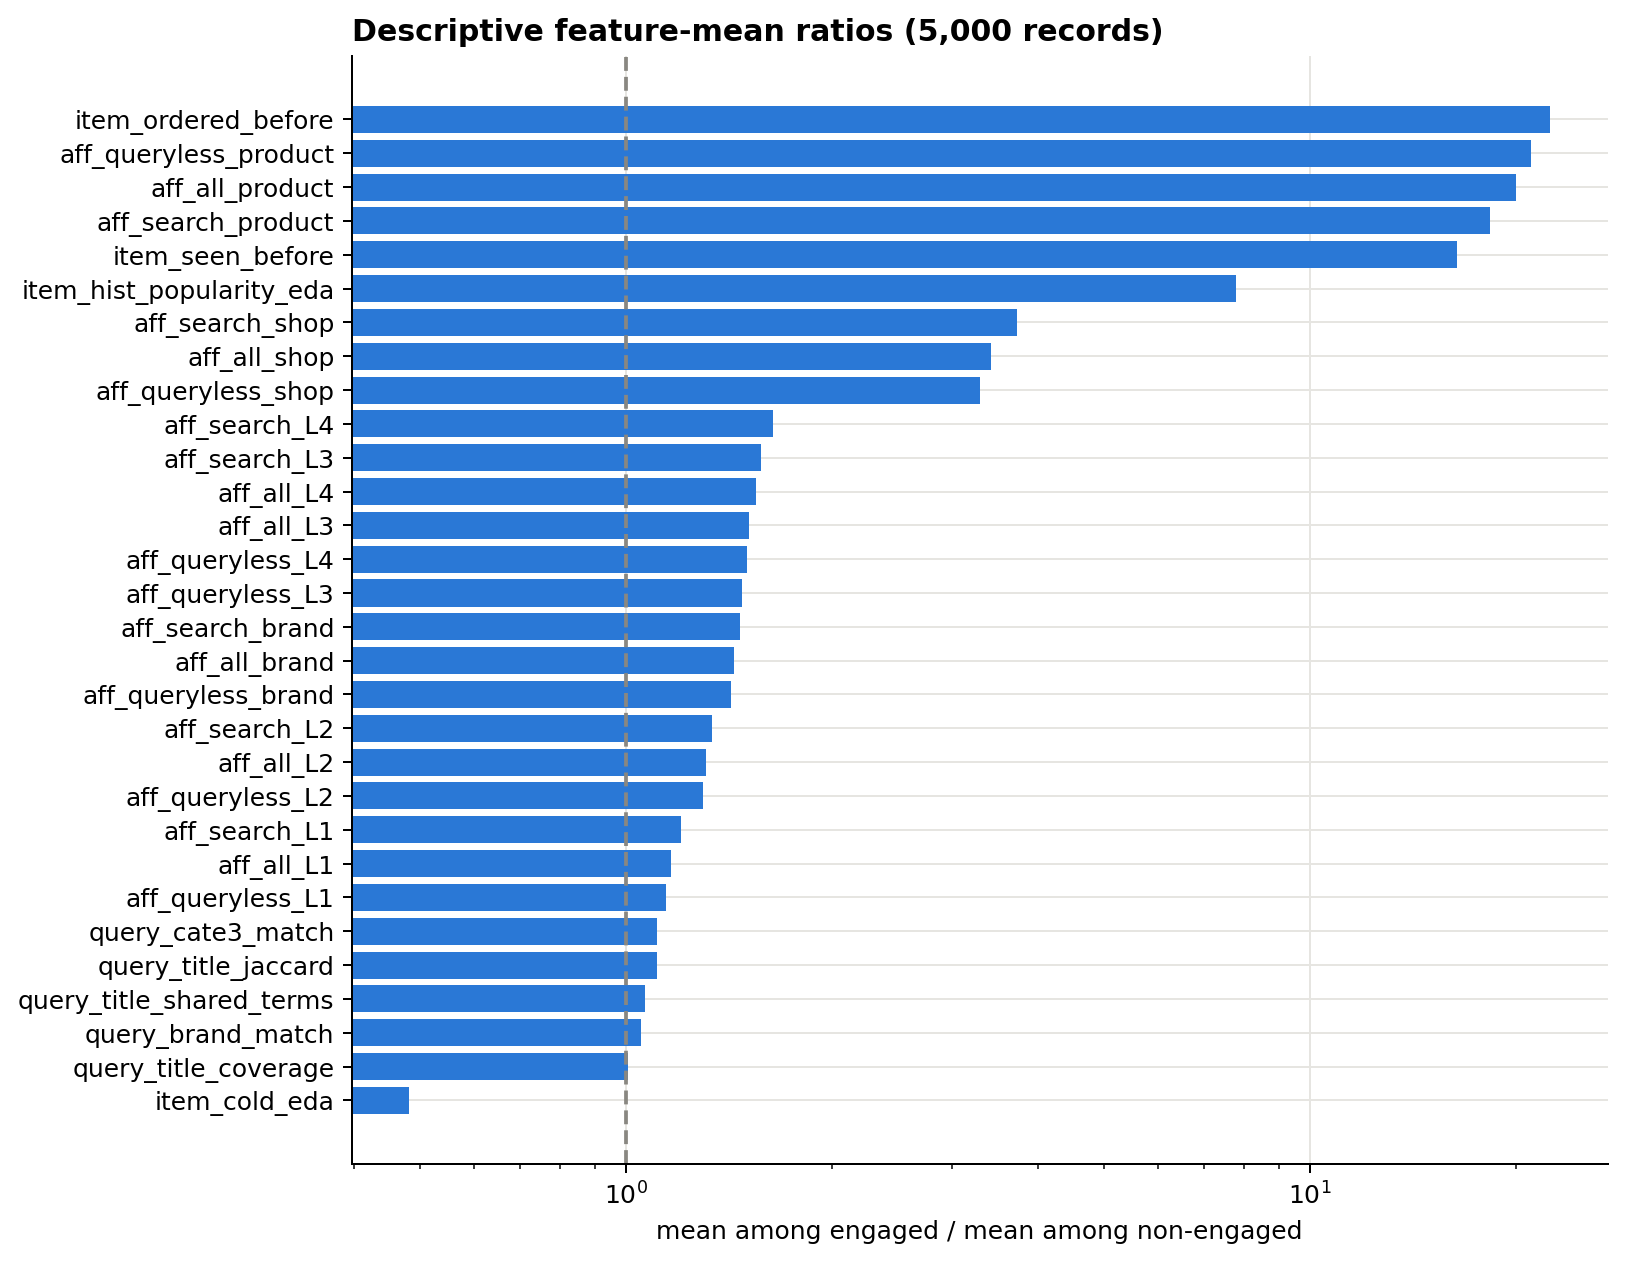
\includegraphics[width=0.75\textwidth]{figures/fig6_feature_ratios.png}
\caption{Feature mean among engaged / non-engaged candidates, log scale (5,000-record sample)}
\end{figure}

\end{document}
